\documentclass[11pt,letterpaper]{article}
\usepackage[utf8]{inputenc}

%%%%%%%%%%%%%%%%%%%%%%%%%%%%%%%%%%%%%%%%%%%%%%%%%%%%%%%%%%%%%%%%%%%%%%%%%
\pagestyle{plain}                                                      %%
%%%%%%%%%% EXACT 1in MARGINS %%%%%%%                                   %%
\setlength{\textwidth}{6.5in}     %%                                   %%
\setlength{\oddsidemargin}{0in}   %% (It is recommended that you       %%
\setlength{\evensidemargin}{0in}  %%  not change these parameters,     %%
\setlength{\textheight}{8.5in}    %%  at the risk of having your       %%
\setlength{\topmargin}{0in}       %%  proposal dismissed on the basis  %%
\setlength{\headheight}{0in}      %%  of incorrect formatting!!!)      %%
\setlength{\headsep}{0in}         %%                                   %%
\setlength{\footskip}{.5in}       %%                                   %%
%%%%%%%%%%%%%%%%%%%%%%%%%%%%%%%%%%%%                                   %%
\newcommand{\required}[1]{\section*{\hfil #1\hfil}}                    %%
\renewcommand{\refname}{\hfil References Cited\hfil}                   %%

%%%%%%%%%%%%%%%%%%%%%%%%%%%%%%%%%%%%%%%%%%%%%%%%%%%%%%%%%%%%%%%%%%%%%%%%%

%PUT YOUR MACROS HERE
% comments: feel free to use your favorable symbol
\usepackage[usenames, dvipsnames]{color}
\usepackage{color,soul}
\usepackage{url}
\usepackage{floatflt,graphicx,color}
\usepackage{epsfig,pstcol,gastex}
\usepackage{subfigure,wrapfig}
\usepackage{clrscode}
\usepackage{amssymb}
\usepackage{amsmath}
\usepackage{verbatim}
\usepackage{alltt}
\usepackage{latexsym}
\usepackage{hyperref}
\usepackage{graphicx}
\usepackage{cite}
\usepackage{todonotes}


\newcommand{\boldstart}[1]{{\noindent \bf #1}}
\newcommand{\boldheading}[1]{{\vspace{0.1in}\noindent \bf #1} \hspace{0.06in}}

\newcommand\PB[1]{\textcolor{blue}{$\spadesuit$\footnote{\textcolor{blue}{$\spadesuit$}\hl{PB: #1}}}}
\newcommand\CF[1]{\textcolor{red}{$\clubsuit$\footnote{\textcolor{red}{$\clubsuit$}\hl{CF: #1}}}}
\newcommand\NB[1]{\textcolor{magenta}{$\bigstar$\footnote{\textcolor{magenta}{$\bigstar$}\hl{NB: #1}}}}


\title{A Really Cool Title that Doesn't Use ``Learning'' or ``Security''}
%\author{Peter Beling, Nicola Bezzo and Cody Fleming}
\date{}

\begin{document}

%\maketitle

% !TEX root = main.tex

\section{Motivation and Objectives}

\begin{itemize}
    \item CPS are increasingly everywhere
    \item many CPS are safety-critical, and a fault can literally kill people
    \item cyber threats and vulnerabilities are increasingly everywhere
    \item {\bf key assertion} traditional defense techniques are not only insufficient, they are at least in some cases unnecessary. This assertion is also true for the different paradigm of what we will call ``cyber resilience'' techniques; i.e. it is unclear whether they are necessary or sufficient
    \item {\bf another key assertion} security techniques for CPS are usually tailored for that specific application or system. There is no assurance when transitioning to other applications or techniques.
    \item therefore, we propose to understand the theory and science behind whether, when, and where different CPS security/resilience techniques are (in)effective and/or (un)necessary
\end{itemize}

\todo{bold statement about the current state of cyber and safety-critical CPS}

Consider the example in Figure~\ref{fig:motivation}, where\todo{catchy example with associated figure}

\begin{wrapfigure}{r}{0.3\linewidth}
	\centering{
		%\includegraphics[width=\linewidth,trim={142px 393px 88px 165px},clip]{figs/}
		\caption{not sure what to put here.}
		\label{fig:motivation}}	
\end{wrapfigure}

Our focus is not on improving defenses against cyber attack, or even improving detection and adaptation techniques in the face of a cyber attack. Rather, our efforts aim to\todo{understand the tradeoffs and optimize decision-making about when, where, and how to apply design patterns...}


Our approach is to develop models that can...
\begin{wrapfigure}{r}{0.6\linewidth}
	\centering{
		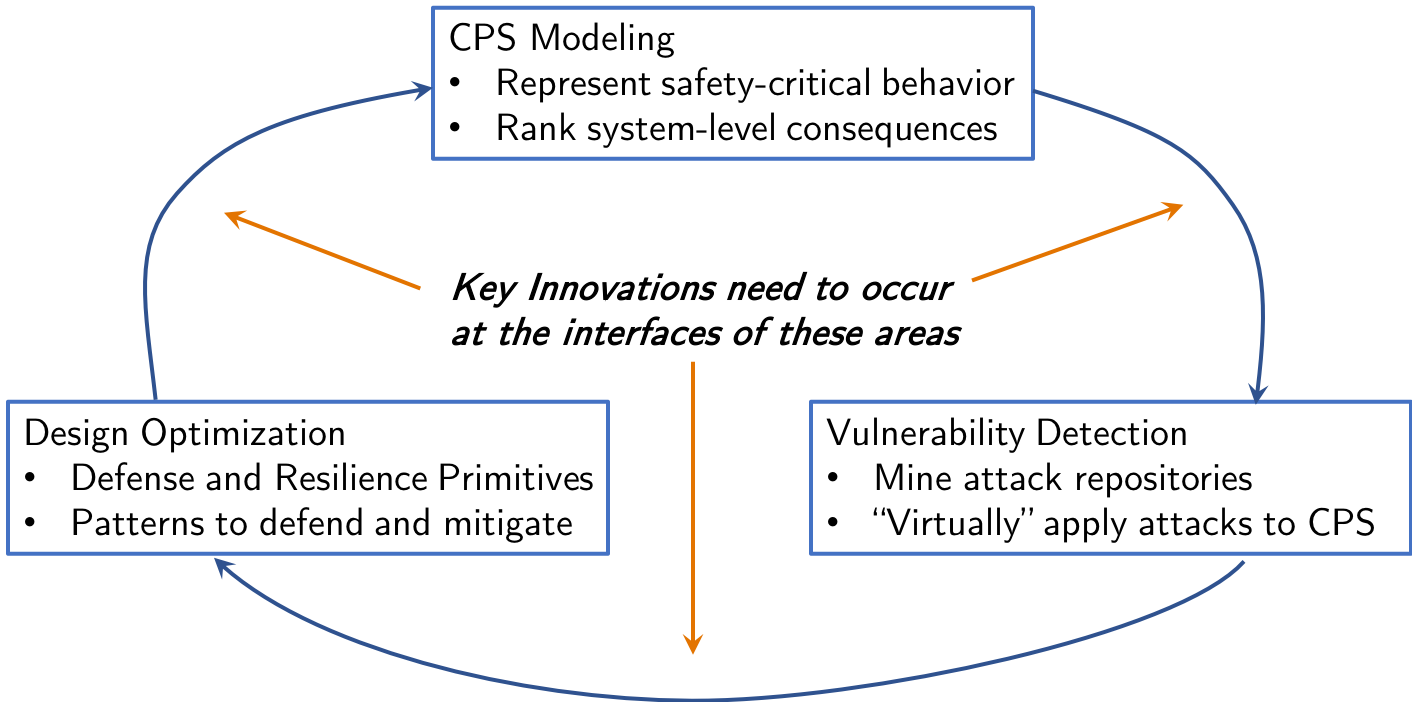
\includegraphics[width=\linewidth,trim={0 0 0 0},clip]{figs/workflow}
		\caption{Overview \hl{this is just notional, needs a good figure}}
		\label{fig:motivation}}	
\end{wrapfigure}

% !TEX root = main.tex

\section{Background and Related Approaches}\label{sec:background}
A bit about traditional defense and its limitations, some of our work (and others') on resilience, etc
\NB{I think we need to pick 1 or more techniques that have been well developed like my resilient state estimator or the resilient kalman filter and use those to both motivate the problem and use them to show how to transition to other applications and platforms}
\NB{I can discuss about these techniques}

\section{Research Goals and Approaches}\label{sec:approach}

We propose to focus on three research thrusts that aim to \todo{1, 2, and 3...}

%%%%%%%%%%%%%%%%%%%%%%%%%%%%%%%%%
\subsection{Thrust 1: ...}

\boldheading{Goals and Challenges:} 

\boldheading{Approaches and Preliminary Work:} 

\boldheading{Future Work:} If successful, this project will extend our preliminary work by\todo{by ``future work'' I mean the work we'll do if this is funded}

\subsection{Thrust 2: ...}

\boldheading{Goals and Challenges:} 

\boldheading{Approaches and Preliminary Work:} 

\boldheading{Future Work:} 

\subsection{Thrust 3: ...}

\boldheading{Goals and Challenges:} 

\boldheading{Approaches and Preliminary Work:} 

\boldheading{Future Work:} 

\section{Integration and Validation Plan}
This multidisciplinary research requires expertise in a number of areas, a tight collaboration among its team members, and a close integration of all phases of the research. The primary expertise needed includes \todo{controls, decision-making, modeling...} The team consists of experts in all of the areas and the rough team breakdown is shown in Figure~\ref{fig:testbed}. The PIs are all members of the Link Lab, whose mission is to enhance excellence of CPS research at the University of Virginia. They and all of their students will be sitting together on a daily basis in a 17,000 square foot collaborative lab. They will formally meet as a group once per week but subgroup meetings and impromptu meetings will take place on a daily basis.

\begin{wrapfigure}{r}{0.3\linewidth}
	\centering{
		%\includegraphics[width=\linewidth,trim={142px 393px 88px 165px},clip]{}
		\caption{Proposed experimental testbed will consist of one ground and two aerial vehicles.}
		\label{fig:testbed}}	
\end{wrapfigure}

While significant research progress will occur in each subproject, we emphasize a rigorous plan for integration throughout the project. This includes a periodic interactive activity called the\todo{something related to exercising our theory on a testbed, which we will describe below. Nicola, do you have boilerplate on the stuff in your lab?}

\boldheading{Timeline and milestones:}

\begin{figure}
    \centering
    \includegraphics{}
    \caption{Timeline of proposedwork, including technical development, evaluation ,and
  broader impact}
    \label{fig:timeline}
\end{figure}

\section{Broader Impact, Education Plan, and Outreach Activites}\label{sec:impacts}

\boldheading{Dissemination:} The proposed research will enhance the ...

\boldheading{Integration into curriculum:} The proposed research will be integrated into coursework

\boldheading{Undergraduate research:}

\boldheading{K-12 outreach:}

\boldheading{Contributions to diversity: }

\section{Relevant Prior Research Funded by NSF}
{\bf Cody Fleming} is Co-PI on NSF grant... . {\bf Peter Beling} is ... . {\bf Nicola Bezzo} ...

\end{document}


%\section*{Introduction}

% A paragraph about: how complex and ubiquitous CPS are becoming, particularly safety-critical CPS. How scary it is that they are vulnerable to cyber-security threats...
\noindent As cyber-physical systems (CPS) increasingly pervade the world and\hl{...jkl}.

%A paragraph about the progress, state-of-the-art, and limitations w/r/t these problems...
\CF{not totally necessary for a white paper, but this could help us figure out what we want to say...}Current approaches to securing CPS can be broken down into (1) perimeter-oriented security, or hardening, that attempts to prevent compromises from happening and (2) resilience-based security that adapts and maintains service in the face of threats and compromises. Both approaches come at a cost and have limitations. There is currently no approach for deciding which components of a CPS need to be secured, with which method(s), given the current state of potential threats. Furthermore, most techniques do not yet handle many classes of threats that do not currently exist.

%do something new and different, with 3 (?) main pillars or thrusts to the work:
We propose to address these limitations and challenges by asking the following fundamental question\CF{more than one?}: \hl{blah blah blah}? We will focus not only on the response of a particular component to a threat or compromise. Rather, we will also focus on the {\em overall system response} relative to its performance objectives and safety constraints. Furthermore, many of the problems in CPS arise out of the interactions not only among components but also among distributed, autonomous agents. How should a system of distributed agents respond to a threat in order to maximize overall system performance while minimizing risk?
To answer these questions, we propose the following thrusts, and perhaps more importantly, the integration and coupling of these thrusts.

\boldheading{Thrust I -- Model-based Representation of Vulnerabilities in CPS}: something akin to a repository of models that can run virtually in parallel with the real CPS. Not exactly like a Gazebo simulator or high-fidelity Simulink model, although that could be helpful. But a set of models that represent operational/performance goals, formalized safety constraints, behavioral models of system (a la Simulink), as well as more ``attackable'' artifacts, like the types of drivers/OS/chips/etc that actually get attacked

%\medskip

\boldheading{Thrust II -- Prediction of Vulnerability}: not a great title, but I am thinking about more general classes/abstractions of threats based on existing or newly obtain data...NLP...matching threats and vulnerabilities to models

%\medskip 

\boldheading{Thrust III -- Adaptation of Operations} what I was thinking here was not just ``resilience'' of an estimator or control system, but resilience of an overall fleet of autonomous systems. E.g. the Grand Canyon example. By the way, I (Cody) am probably thinking of this in more of a real-time / tactical way than Peter might be, where you are thinking more strategically (longer time horizon) about what to do if you get new information about a class of threats. Perhaps there is no distinction, but if there is, I am confident we can merge/converge...

% NOTES from 24 April
Platforms
\begin{enumerate}
    \item study the exact same platform, in the exact same configuration, but in a different context (with different risks / consequences)
    \item study the same platform, new configuration, same context as original (and maybe a new one with different risks / consequences)
    \item ...
    \item translate to new platform, new context, but one attack is common between two (this is the toughest)
\end{enumerate}

Preliminary work
\begin{itemize}
    \item taxonomy of attacks and how they work on various CPS components
    \item adaptation at control level and detection via state estimation
\end{itemize}

% there are techniques for detecting attacks; we will collect them
% we have a way of ``correctly'' modeling systems
% two levels
%   1. soft method that frames a set of technical questions. i have learned from past / existing attacks on other systems; how do they apply to the systems i am trying to put out there
%   2. pulling from libraries of mitigations

% the notion of security is wrong; the notion of consuming the other guy's resources is the right way to go...or introducing uncertainty into his world


% from CPS call
% CPS Security: What makes CPS security different from traditional cyber security? Are there new directions, or does CPS introduce new risks, at the intersection of the cyber and physical space that promise higher levels of security than those obtained by purely physical or cyber methods? What new protections and defenses are afforded through the interactions among the cyber and physical components of a CPS?


%\end{document}
